\documentclass{beamer}
\usepackage{lmodern}
\usepackage[utf8]{inputenc}

\usepackage{enumerate}
\usepackage{multimedia}

\usetheme{polimix}
\graphicspath{{./immagini}} 

\title{Progetto di Modelli e metodi per l'inferenza statistica}
%\subtitle{subtitle}
%nomi in ordine alfabetico per cognome
\author{Pietro Masini, Giulia Riccardi, Sofia Sannino, Alessandro Wiget }
%\supervisor{Supervisor}{supervisor name}
%aggiungere fonte dei dati
\institute{Politecnico di Milano}
%\coadvisor{Co-Advisor}{co advisor name}
\date[05/06/2024]{5 Giugno 2024}

\begin{document}

%%%%%%%%%%%%%%%%%%%%%%%%%%%%%%%%%%%%%%%%%%%%%%%%%%%%%%%%%%%%%%%%%%%%%%%%%%%%%%%%%%%%%%%%%%%%%%%%%%%%%%%%%%%%%%%%%%%%

\begin{frame}
\titlepage
\end{frame}

\addtocounter{framenumber}{-1}

%%%%%%%%%%%%%%%%%%%%%%%%%%%%%%%%%%%%%%%%%%%%%%%%%%%%%%%%%%%%%%%%%%%%%%%%%%%%%%%%%%%%%%%%%%%%%%%%%%%%%%%%%%%%%%%%%%%%

\begin{frame}
\frametitle{Obiettivo}
\text{Vogliamo costruire un modello in grado di prevedere la probabilità} \\
\text{di dropout di uno studente di ingegneria matematica al termine del}
\text{primo semestre del primo anno.}

\tableofcontents
\end{frame}


%%%%%%%%%%%%%%%%%%%%%%%%%%%%%%%%%%%%%%%%%%%%%%%%%%%%%%%%%%%%%%%%%%%%%%%%%%%%%%%%%%%%%%%%%%%%%%%%%%%%%%%%%%%%%%%%%%%
\begin{frame}
\frametitle{Il modello}
\text{Scelta di un modello di regressione logistica:}\\
$Y_{i} \sim Be(p_{i})$\\
$\log\left(\frac{p_{i}}{1-p_{i}}\right) = Z\underline{b}$ \\
dove $Z$ è la matrice disegno e $\underline{b}$ è il vettore dei parametri.

\end{frame}
%%%%%%%%%%%%%%%%%%%%%%%%%%%%%%%%%%%%%%%%%%%%%%%%%%%%%%%%%%%%%%%%%%%%%%%%%%%%%%%%%%%%%%%%%%%%%%%%%%%%%%%%%%%%%%%%%%%
\begin{frame}
    \frametitle{Analisi esplorativa}
    \text{Il nostro dataset è del Politecnico di Milano e presenta covariate} 
    \text{sia numeriche che categoriche.}
    %immagine dataset
    \text{Notiamo che ci sono persone che non hanno iniziato il corso e }
    \text{in più ci sono persone che sono iscritte da 3 anni e mezzo o più.}
\end{frame}

\begin{frame}
    \frametitle{Analisi esplorativa e selezione degli studenti}
    \begin{figure}[h]
    \centering
    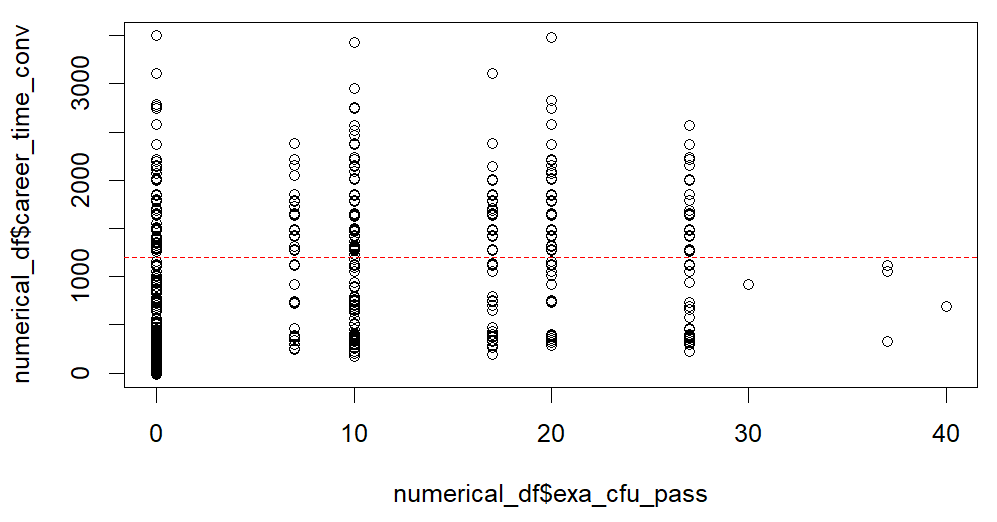
\includegraphics[width=1\textwidth]{Screenshot 2024-05-26 123827.png} % Adjust the width as needed
    \label{}
\end{figure}
    
\end{frame}



\begin{frame}
\frametitle{Correlazioni tra le covariate numeriche}
\begin{figure}[h]
    \centering
    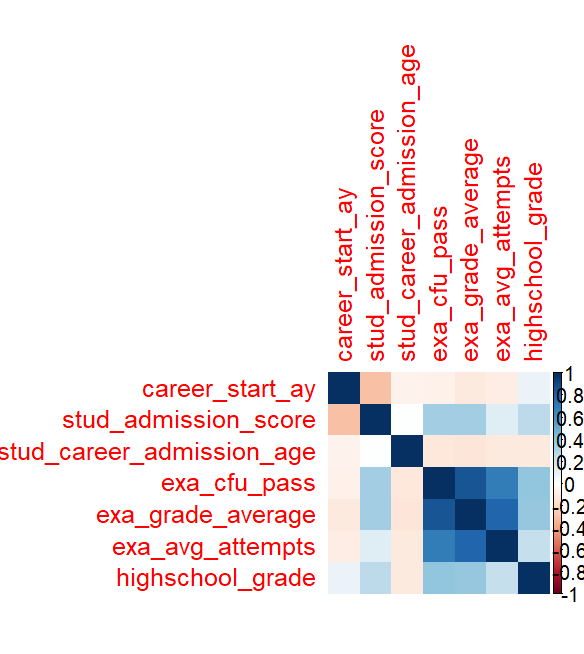
\includegraphics[width=.7\textwidth]{Rplot.png} % Adjust the width as needed
    \label{Tabella delle correlazioni}
\end{figure}
\end{frame}

\begin{frame}
\frametitle{}
\begin{figure}[h]
    \centering
    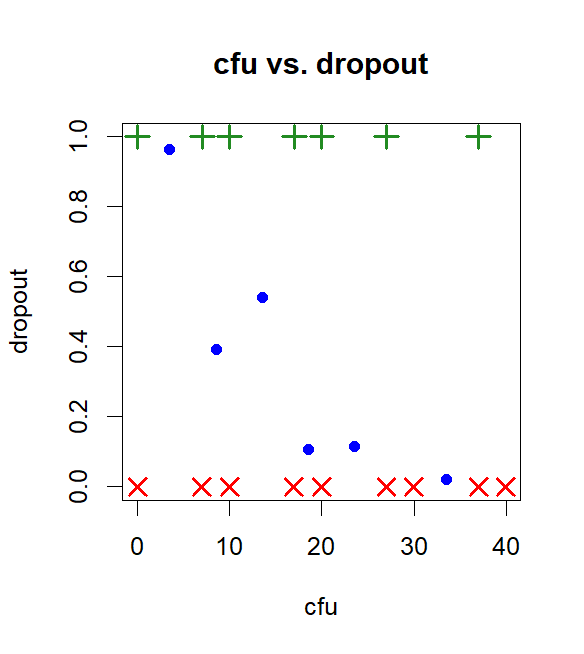
\includegraphics[width=.75\textwidth]{Rplot01.png} % Adjust the width as needed
    \label{}
\end{figure}
\end{frame}
%%%%%%%%%%%%%%%%%%%%%%%%%%%%%%%%%%%%%%%%%%%%%%%%%%%%%%%%%%%%%%%%%%%%%%%%%%%%%%%%%%%%%%%%%%%%%%%%%%%%%%%%%%%%%%%%%%%
\begin{frame}
\frametitle{Prima regressione logistica}
\begin{figure}[h]
    \centering
    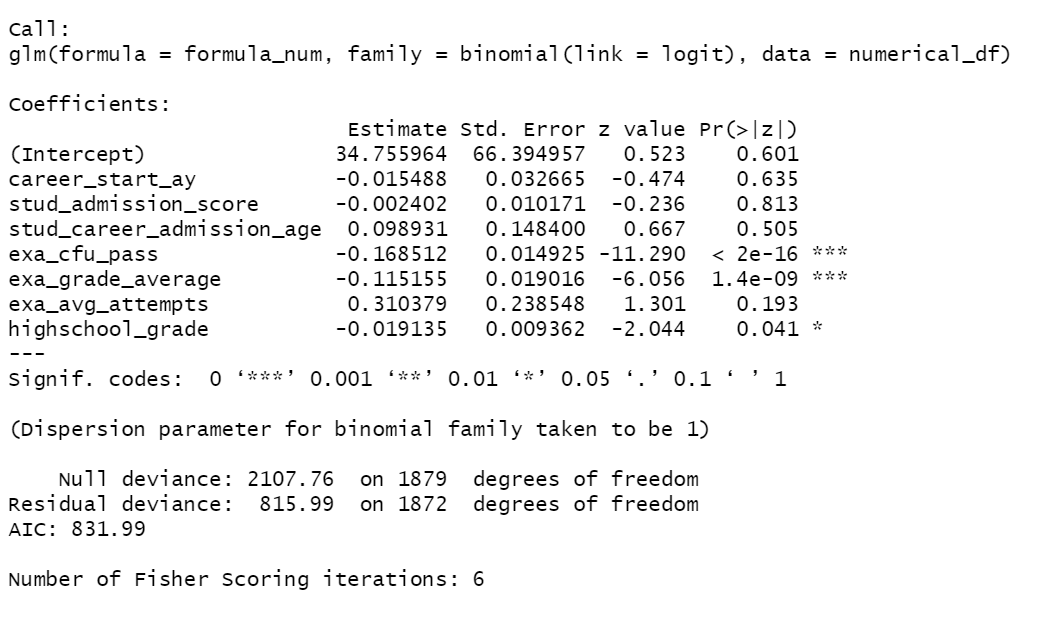
\includegraphics[width=1.1\textwidth]{Screenshot 2024-05-26 115620.png} % Adjust the width as needed
    \label{Prima regressione con tutte le covariate numeriche}
\end{figure}
\end{frame}


\begin{frame}
\frametitle{Odds Ratio delle covariate più significative}
\begin{flushleft}
    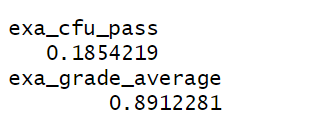
\includegraphics[width=.5\textwidth]{Screenshot 2024-05-26 120049.png} % Adjust the width as needed
    
\end{flushleft}

\text{Se uno studente acquisisce 10 cfu in più,}
\text{il rischio di dropout diminuisce dell'$80\%$.}\\[.7cm]
\text{Inoltre, il rischio di dropout diminuisce del $10\%$}
\text{all'aumentare di un punto di media.}

\end{frame}

\begin{frame}
\frametitle{Selezione del modello tramite backward selection}
\begin{figure}[h]
    \centering
    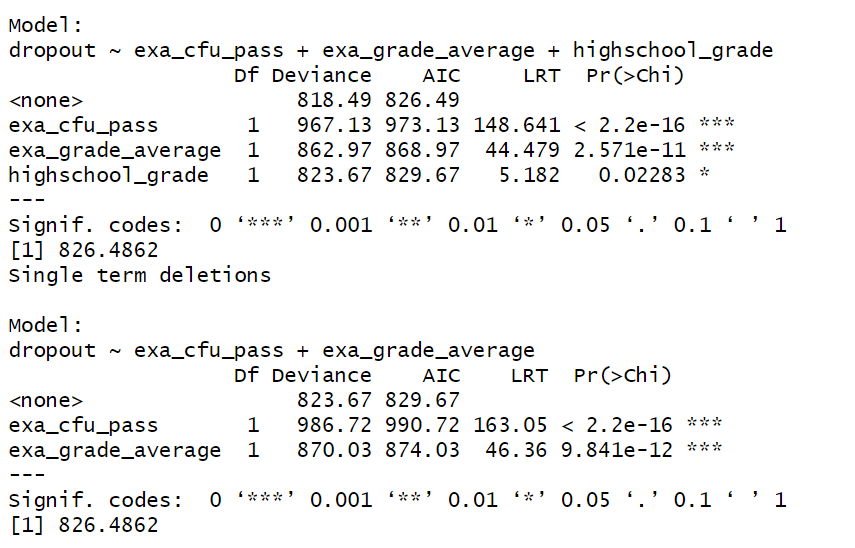
\includegraphics[width=1\textwidth]{Screenshot 2024-05-26 120454.png} % Adjust the width as needed
    \label{}
\end{figure}

\end{frame}

\begin{frame}
\frametitle{Modello finale con covariate numeriche}
\begin{figure}[h]
    \centering
    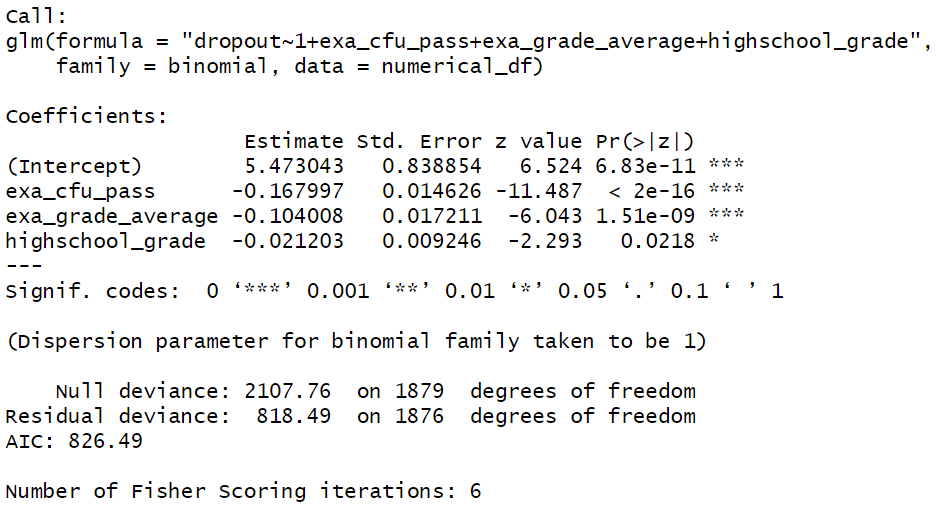
\includegraphics[width=1.07\textwidth]{Screenshot 2024-05-26 120822.png} % Adjust the width as needed
    \label{}
\end{figure}
\end{frame}


\begin{frame}
\frametitle{Introduzione interazione tra le covariate numeriche}
\begin{figure}[h]
    \centering
    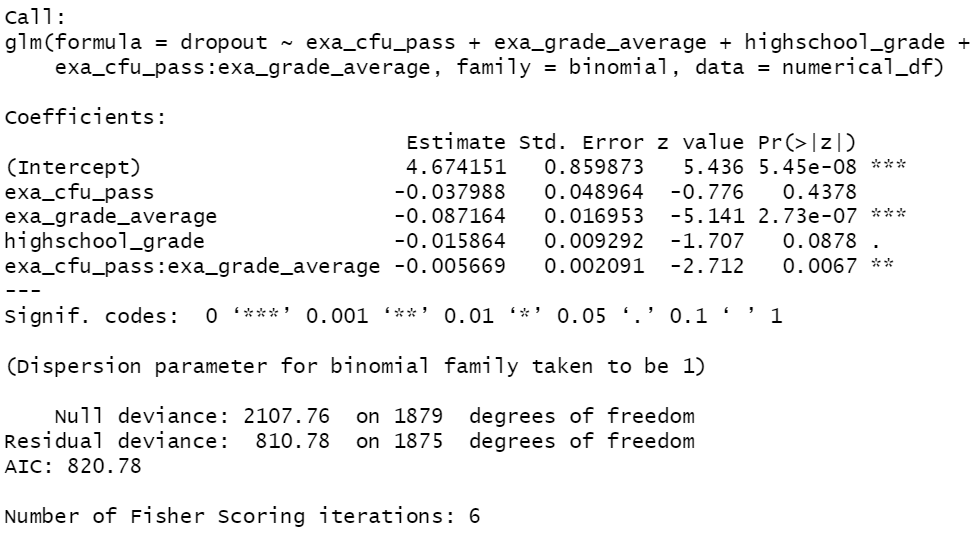
\includegraphics[width=1.07\textwidth]{Screenshot 2024-05-26 121019.png} % Adjust the width as needed
    \label{}
\end{figure}

\end{frame}

\begin{frame}
\frametitle{Introduzione variabili categoriche}
\begin{figure}[h]
    \centering
    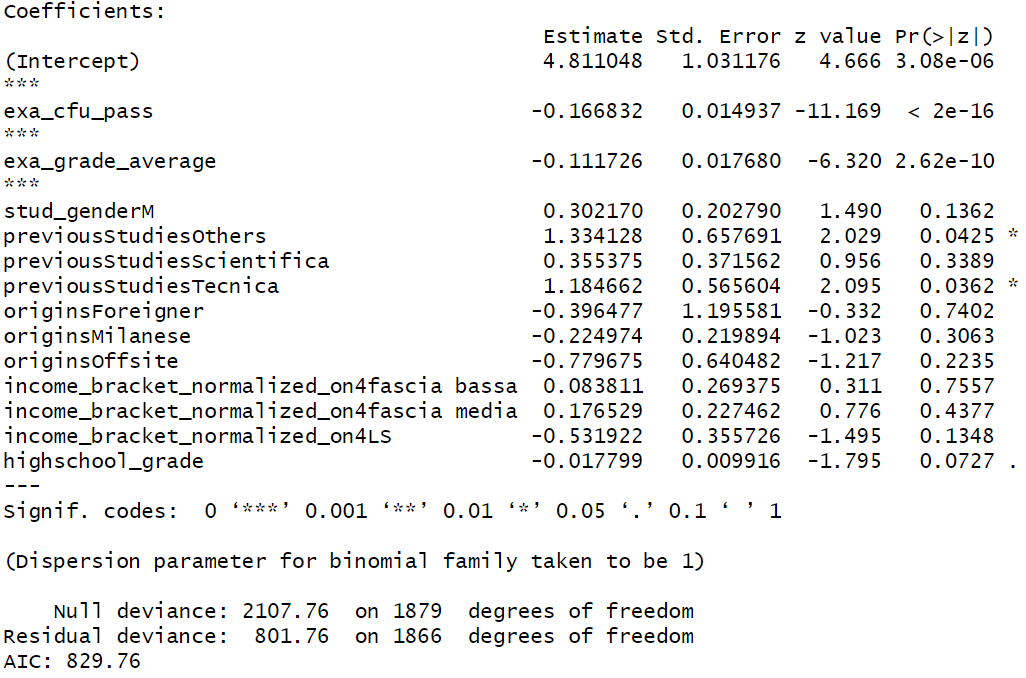
\includegraphics[width=1.07\textwidth]{Screenshot 2024-05-26 121359.png} % Adjust the width as needed
    \label{}
\end{figure}

\end{frame}


\begin{frame}
\frametitle{Backward selection}
\text{Tramite una backward selection, sono state selezionate le}
\text{covariate significative.}
\text{E' emerso che nessuna covariata categorica è significativa.}
\text{Il modello ottimale rimane quello con le sole numeriche.}
\end{frame}

\begin{frame}
\frametitle{Classificazione, curva ROC, confusion matrix}
\begin{figure}[h]
    \centering
    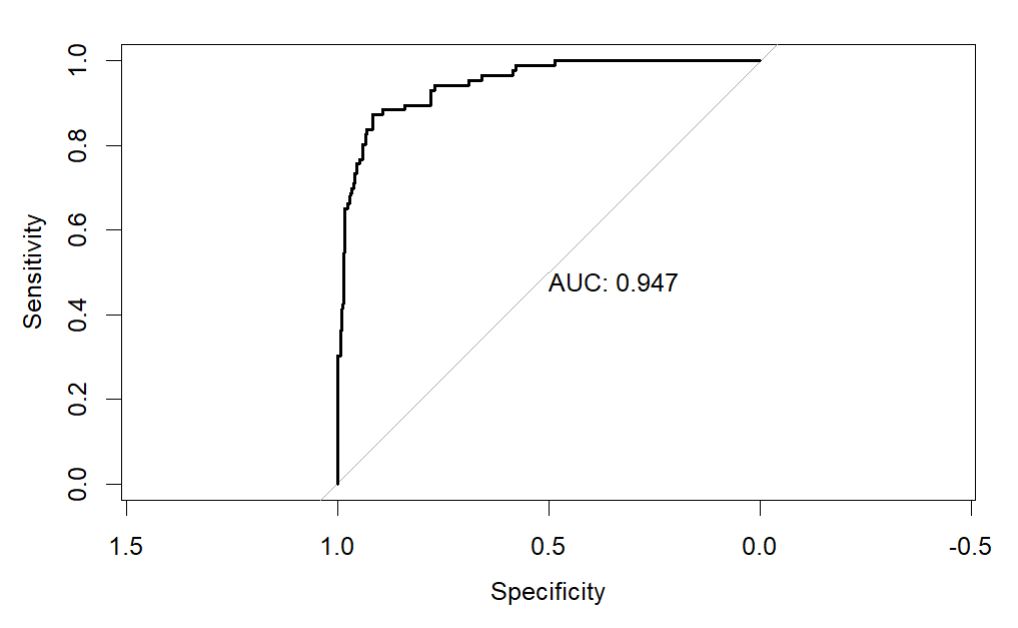
\includegraphics[width=1\textwidth]{Screenshot 2024-05-26 122028.png} % Adjust the width as needed
    \label{}
\end{figure}
\text{Soglia ottimale: 0.2181341}
\end{frame}

\begin{frame}
\frametitle{Classificazione, curva ROC, confusion matrix}
\begin{figure}[h]
    \centering
    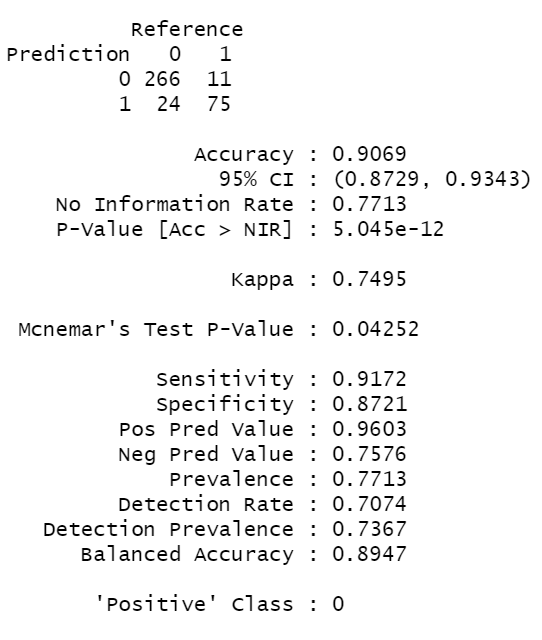
\includegraphics[width=.7\textwidth]{Screenshot 2024-05-26 122256.png} % Adjust the width as needed
    \label{}
\end{figure}

\end{frame}

\begin{frame}

\frametitle{Predizione sugli studenti in corso}

\text{Usando il valore soglia arrontondato e il modello ottimale costruito,}
\text{la probabilità predetta sugli studenti attivi è circa del $37 \%$.}

\end{frame}
%%%%%%%%%%%%%%%%%%%%%%%%%%%%%%%%%%%%%%%%%%%%%%%%%%%%%%%%%%%%%%%%%%%%%%%%%%%%%%%%%%%%%%%%%%%%%%%%%%%%%%%%%%%%%%%%%%%%




%%%%%%%%%%%%%%%%%%%%%%%%%%%%%%%%%%%%%%%%%%%%%%%%%%%%%%%%%%%%%%%%%%%%%%%%%%%%%%%%%%%%%%%%%%%%%%%%%%%%%%%%%%%%%%%%%%%%



%%%%%%%%%%%%%%%%%%%%%%%%%%%%%%%%%%%%%%%%%%%%%%%%%%%%%%%%%%%%%%%%%%%%%%%%%%%%%%%%%%%%%%%%%%%%%%%%%%%%%%%%%%%%%%%%%%%%

%fonti all'inizio o alla fine????
\begin{frame}
\frametitle{Fonti}


\end{frame}


%%%%%%%%%%%%%%%%%%%%%%%%%%%%%%%%%%%%%%%%%%%%%%%%%%%%%%%%%%%%%%%%%%%%%%%%%%%%%%%%%%%%%%%%%%%%%%%%%%%%%%%%%%%%%%%%%%




\end{document} 
